\documentclass{article}
\usepackage[utf8]{inputenc}
\usepackage{caption}
\usepackage{amsmath}
\usepackage{amssymb}
\usepackage{mathtools}
\usepackage{multicol}
\usepackage{graphicx}
\usepackage{wrapfig}
\usepackage{float}
\usepackage[makeroom]{cancel}
\usepackage{mhchem}
\usepackage{pst-plot}

\graphicspath{ {../images/} }

\renewcommand{\familydefault}{\sfdefault}
\renewcommand{\baselinestretch}{1.5} % line spacing
\newcommand{\fline}{\par\noindent\rule{\textwidth}{0.1pt}} % horizontal line (wide)

\title{Topic 8 - Redox Reactions\\Lesson 5 - Electrolysis}
\author{Peter Zhang}

\begin{document}

\maketitle
\tableofcontents
\newpage

\section{Factor Effecting the Amount of Product in Electrolysis}
\begin{itemize}
\item amount of product at the electrodes depends on the qunatity of electric charge passed through the cell

\ce{Q=It} \begin{itemize}\item I = current (A) \item t = time (s) \item Q = charge (C/coulombs) \item 1 mole = 96500C (Faraday's constant) \end{itemize}

\subsection{Example}
How many grams of lead are deposited on the cathode of an electrlyte cell containing \ce{PbBr2 (l)} if a current of $4.3A$ runs through it for 11s?

\begin{align*}
Q&=It\\&=4.3*11\\
&=47.3C\\
&Dividing\ the\ value\ by\ Faraday's\ Constant\\
&=\frac{47.3C}{96500C/mol}\\
&n=0.00049mol\\
\\
\ce{PbBr2}&\rightarrow \ce{Pb2+ + 2Br-}\\
n_{\ce{PbBr2}} &= 0.00049mol
\end{align*}

Since there is a 1:1 ratio of \ce{PbBr2} to \ce{Pb2+}, there is the same number. MOLAR RATIOS come in clutch :)

\item \textbf{Time and current} is directly proportional to the mols created.

\subsection{Electrolysis Example}
\begin{figure}
\centering
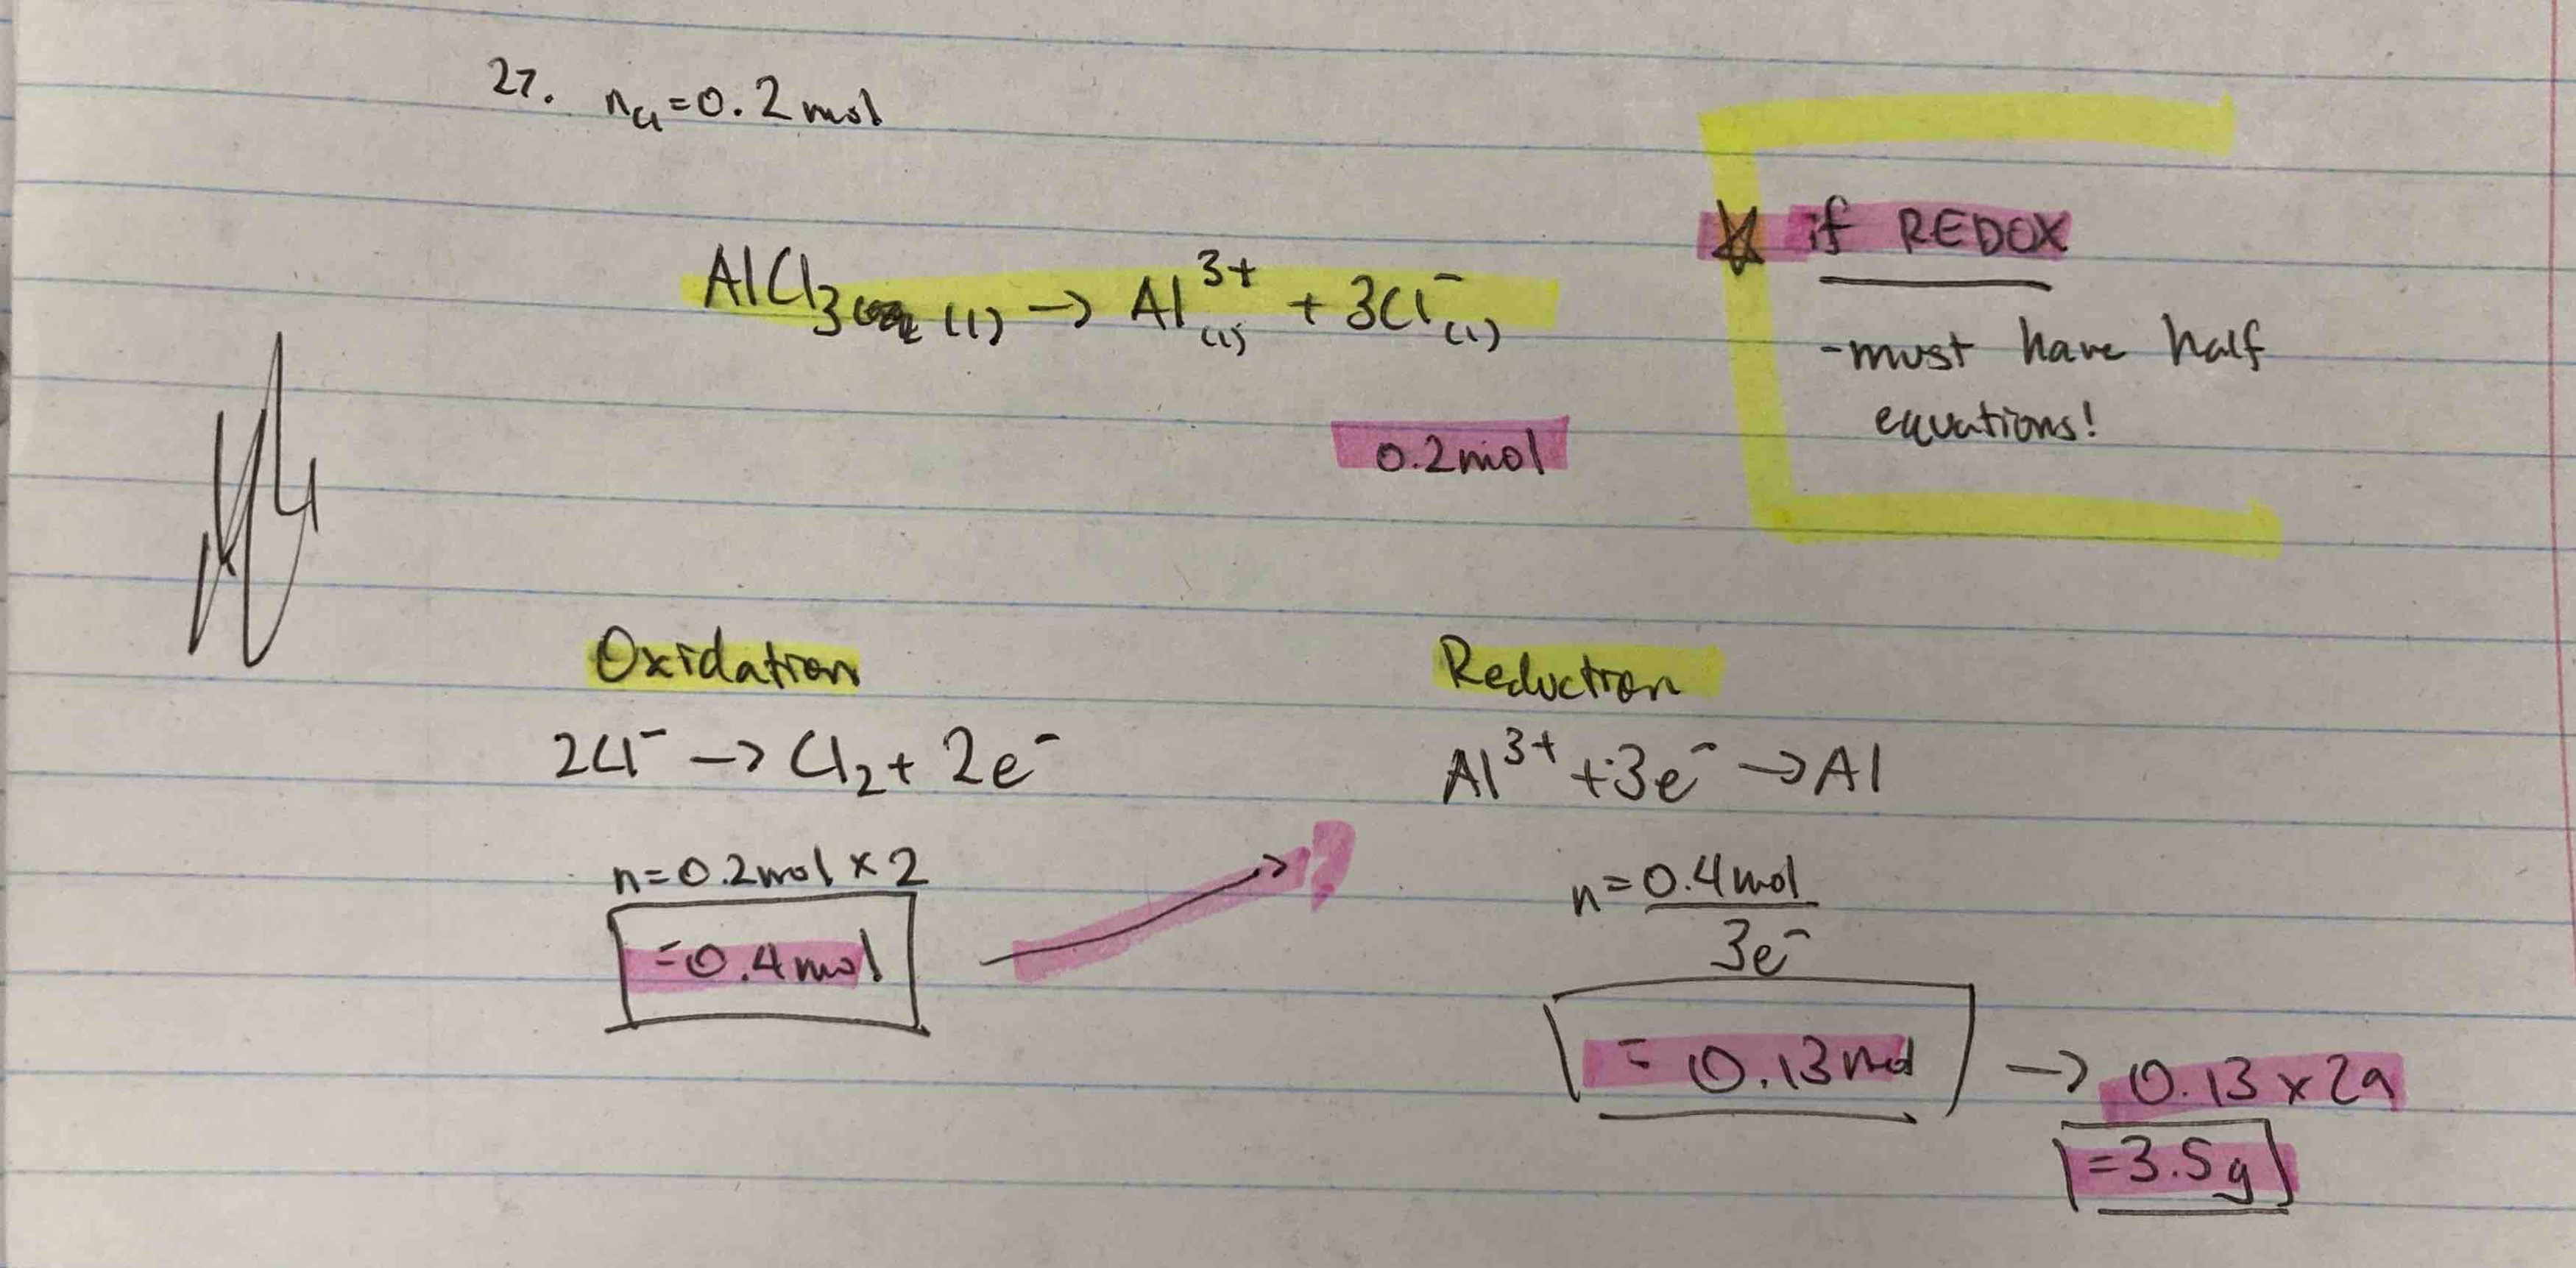
\includegraphics[width=\textwidth]{5.5fig1.JPG}
\captionof{figure}{Sample Electrolysis of AlCl3 (finding mols)}
\end{figure}
\end{itemize}








\end{document}